\documentclass[a4paper,12pt]{article}

% Pakete
\usepackage[utf8]{inputenc}
\usepackage[english]{babel} % Deutsche Sprache
\usepackage{graphicx} % Für Bilder
\usepackage{amsmath} % Für mathematische Formeln
\usepackage{booktabs} % Für Tabellen
\usepackage[hidelinks]{hyperref} % Für Hyperlinks
\usepackage{listings} % Für Code-Blöcke
\usepackage{minted} % Auch für Code-Blöcke
\usepackage{caption}
\usepackage{menukeys}
\usepackage{float}
\usepackage{enumitem}
\usepackage{tocloft}
\usepackage{pgfplots}
\usepackage{pgfplotstable}
\usepgfplotslibrary{groupplots}
\usepackage{siunitx}
\usepackage{multicol}
\usepackage{xcolor}
\usepackage{tikz}
\usepackage{textcomp}
\newcommand{\mytexttilde}{\raisebox{0.5ex}{\texttildelow}}

\usepackage{fancyhdr}
\pagestyle{fancy}

\fancyhf{} % löscht alle aktuellen Kopf- und Fußzeilen

% Kopfzeile: linke Seite = aktuelle Section
\fancyhead[L]{\nouppercase{\leftmark}}

% Fußzeile: linke Seite = Name, rechte Seite = FH Salzburg, zentriert = Seitenzahl
\fancyfoot[L]{Marc Toiflhart, Sebastian Maier}
\fancyfoot[C]{\thepage}
\fancyfoot[R]{Högskolan i Halmstad}

\usepackage{placeins}

\usepackage[
backend=biber,
style=ieee,
sorting=ynt
]{biblatex}

\renewcommand{\listingscaption}{Sourcecode}

\addbibresource{literatur.bib}

\begin{document}

\begin{titlepage}
    \centering
    
\includegraphics[width=5cm]{Resources/hogskolan-halmstad-logo.png} \\[0.5cm] % Logo
    Högskolan i Halmstad \\[0.2cm]
    Biometric Recognition \\[1.5cm]
    
    \hrule
    \vspace{0.4cm} % statt \\[0.4cm]
    {\LARGE \textbf{Laboratory Report}}
    \vspace{0.4cm}
    \hrule
    \vspace{1.5cm} % statt \\[1.5cm]

    {\Large \textbf{Biometric Recognition Laboratory}} \\[0.2cm]
    {\Large Hand Geometry} \\[1cm]
    
    \textbf{Author:} Marc Toiflhart, Sebastian Maier \\[0.2cm]
    \textbf{Date:} \today \\[0.2cm]
    \textbf{Supervisor:} Kevin Hernández Diaz

    \vfill
\end{titlepage}
\newpage

% Inhaltsverzeichnis
\tableofcontents
\newpage

% Abbildungsverzeichnis
\listoffigures
\newpage

% Tabellenverzeichnis
\listoftables
\newpage


\begin{center}
    \textbf{Summary}
\end{center}

\noindent
This laboratory session focused on the implementation and evaluation of a biometric recognition system based on \textbf{hand geometry}. Individual hand measurements were taken and processed into feature vectors, which were then used to construct a reference vector through averaging and a test vector for verification.

\vspace{0.3em}
\noindent
The system was evaluated in both \textbf{identification mode} (one-to-many comparison) and \textbf{verification mode} (one-to-one comparison) using the Euclidean distance metric. Key performance indicators such as the \emph{rank-based probability function} $P(k)$, the \emph{Cumulative Match Characteristic (CMC)} curve, \emph{False Rejection Rate (FRR)}, \emph{False Acceptance Rate (FAR)}, and the \emph{Equal Error Rate (EER)} were calculated and visualized.

\vspace{0.3em}
\noindent
Threshold values were analyzed to explore the trade-off between \textbf{security} (minimizing FAR) and \textbf{convenience} (minimizing FRR).

\newpage
\section{Measure hand properties}
%Aufgabenstellung:
Measure in each image provided, the hand geometry properties (finger’s length and width, palm width, etc.) according to the "measuring template" attached with the exercise. Use a ruler and measure in mm, e.g. 20 mm. You will then obtain four feature vectors E1, E2, E3 and E4, one for each image.


\section{Identification exercise}

\subsection{Calculating P(k) by hand}
%Aufgabenstellung:
Calculate by hand the function P (k) for k = 1, 2, ....P (k) indicates the chance (probability) that the correct identity is output in position k of IdLista. Draw the function P(k) that you calculated in a graph.

\subsection{Calculating TPIR (M) and plotting CMC curve}
%Aufgabenstellung:
Calculate by hand the function TPIR (M) and draw it in a graph (the CMC curve). 
TPIR (M) indicates the chance (probability) that the correct identity is output in the first M positions of the output list.  TPIR (M) is obtained by summing up P(k) up to k = M.
Put also the values of P (k) and TPIR (M) in a table.


\subsection{List Length for 90\% Identification Probability}
%Aufgabenstellung:
From TPIR (M), calculate the length of the list M to have a 90\% chance that the correct identity is obtained in IdLista among the first M identities.

\subsection{Most and Least Similar IDs with Distances}
%Aufgabenstellung:
Find the two ID numbers that are the most and the least similar to your own ID. Also write down the distances of the two cases (how similar the hands are).


\section{Verification Exercise}

\subsection{FAR and FRR Calculation from Genuine and Impostor Distances}

\noindent
In this exercise, the verification performance of the biometric system was evaluated by analyzing distances between test and reference vectors for \textbf{genuine} (same person) and \textbf{impostor} (different person) comparisons.

\vspace{0.5em}
\noindent
Using the previously calculated distance vectors:
\begin{itemize}[noitemsep]
    \item \texttt{ShDist} — distances for genuine pairs (true claims)
    \item \texttt{OhDist} — distances for impostor pairs (false claims)
\end{itemize}

\noindent
we computed the \textbf{False Rejection Rate (FRR)} and \textbf{False Acceptance Rate (FAR)} for a range of threshold values. These two metrics express the likelihood of two types of errors:

\begin{itemize}[noitemsep]
    \item \textbf{FRR} — the probability that a genuine user is incorrectly rejected
    \item \textbf{FAR} — the probability that an impostor is incorrectly accepted
\end{itemize}

\vspace{0.5em}
\noindent
The following MATLAB code was used to perform the calculation:

\begin{minted}[fontsize=\small, linenos]{matlab}
[ShDist, OhDist] = DistNew('eucl', DB, TEST);

th = linspace(0, 15, 200);
N_th = length(th);

FRR = zeros(1, N_th);
FAR = zeros(1, N_th);
FR_count = zeros(1, N_th);
FA_count = zeros(1, N_th);

for i = 1:N_th
    FR_count(i) = sum(ShDist > th(i));       % False Rejections
    FRR(i) = FR_count(i) / numel(ShDist);    % FRR = FR / genuine total

    FA_count(i) = sum(OhDist <= th(i));      % False Acceptances
    FAR(i) = FA_count(i) / numel(OhDist);    % FAR = FA / impostor total
end

FRRTable = table(th', FR_count', FRR', ...
    'VariableNames', {'Threshold', 'FR_Errors', 'FRR'});
FARTable = table(th', FA_count', FAR', ...
    'VariableNames', {'Threshold', 'FA_Errors', 'FAR'});
\end{minted}

\vspace{0.5em}
\noindent
This results in a table showing, for each threshold:
\begin{itemize}[noitemsep]
    \item Number of false rejections and false acceptances
    \item Corresponding FRR and FAR probabilities
\end{itemize}

\vspace{0.5em}
\noindent
An excerpt from the resulting table is shown below:

\vspace{1em}
\begin{table}[H]
\centering
\begin{tabular}{@{}rrr@{}}
\toprule
\textbf{Threshold} & \textbf{FR Errors} & \textbf{FRR} \\
\midrule
0.00000  & 40 & 0.95238 \\
0.07538  & 40 & 0.95238 \\
0.15075  & 40 & 0.95238 \\
0.22613  & 40 & 0.95238 \\
0.30151  & 40 & 0.95238 \\
0.52764  & 40 & 0.95238 \\
0.60302  & 39 & 0.92857 \\
0.75377  & 38 & 0.90476 \\
0.97990  & 37 & 0.88095 \\
1.28140  & 34 & 0.80952 \\
1.50750  & 30 & 0.71429 \\
1.80900  & 24 & 0.57143 \\
2.26130  & 17 & 0.40476 \\
2.86430  & 10 & 0.23810 \\
3.31660  &  6 & 0.14286 \\
3.84420  &  5 & 0.11905 \\
4.44720  &  4 & 0.09524 \\
5.27640  &  3 & 0.07143 \\
5.80400  &  1 & 0.02381 \\
6.63320  &  0 & 0.00000 \\
\bottomrule
\end{tabular}
\caption{Excerpt from False Rejection Rate (FRR) table for various thresholds}
\label{tab:frr_table}
\end{table}

\vspace{1em}
\begin{table}[H]
\centering
\begin{tabular}{@{}rrr@{}}
\toprule
\textbf{Threshold} & \textbf{FA Errors} & \textbf{FAR} \\
\midrule
0.00000  & 0   & 0.00000 \\
0.45226  & 0   & 0.00000 \\
2.11060  & 2   & 0.00116 \\
2.63820  & 5   & 0.00290 \\
3.24120  & 7   & 0.00406 \\
3.91960  & 24  & 0.01394 \\
4.89950  & 59  & 0.03426 \\
5.65330  & 107 & 0.06214 \\
6.63320  & 186 & 0.10801 \\
7.83920  & 295 & 0.17131 \\
9.12060  & 423 & 0.24564 \\
10.47700 & 568 & 0.32985 \\
11.68300 & 683 & 0.39663 \\
12.73900 & 780 & 0.45296 \\
13.94500 & 899 & 0.52207 \\
15.00000 & 991 & 0.57549 \\
\bottomrule
\end{tabular}
\caption{Excerpt from False Acceptance Rate (FAR) table for various thresholds}
\label{tab:far_table}
\end{table}

\vspace{0.5em}
\noindent
To visualize the relationship between FRR and FAR over the threshold range, the following plot was generated:

\begin{figure}[H]
    \centering
    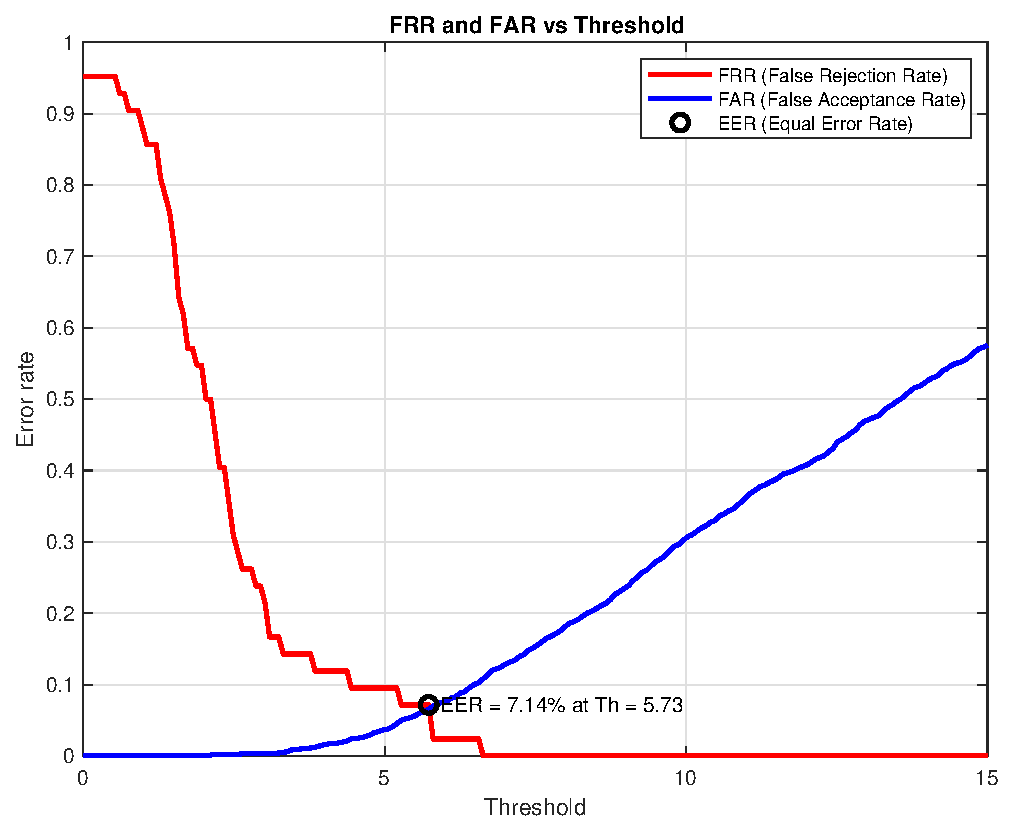
\includegraphics[width=0.8\textwidth]{figures/eer_plot.eps}
    \caption{FRR and FAR vs. threshold. The intersection indicates the Equal Error Rate (EER).}
    \label{fig:frr_far_curve}
\end{figure}

\vspace{0.5em}
\noindent
As shown in \autoref{fig:frr_far_curve}, the False Rejection Rate (FRR) decreases while the False Acceptance Rate (FAR) increases with rising threshold values. This reflects the typical trade-off between \textbf{security} and \textbf{convenience} in biometric verification systems:

\begin{itemize}[noitemsep]
    \item At low thresholds, only very similar feature vectors are accepted — reducing FAR (high security), but increasing FRR (low user convenience).
    \item At high thresholds, more variability is tolerated — reducing FRR (high convenience), but increasing FAR (security risk).
\end{itemize}

\noindent
The point at which the FRR and FAR curves intersect is known as the \textbf{Equal Error Rate (EER)}. It represents a threshold where both types of errors occur at the same probability, providing a balanced trade-off between rejecting genuine users and accepting impostors. 

\vspace{0.5em}
\noindent
A lower EER value indicates a more accurate and reliable biometric system. In this experiment, the EER occurred at a threshold of \SI{5.73}{} with an error rate of approximately \SI{7.14}{\percent}.


\subsection{FR Error Calculation and Threshold Variation}

\noindent
In this section, we analyze how the number of \textbf{False Rejection (FR)} errors varies with different threshold values. A \textbf{false rejection} occurs when a genuine user's biometric sample is mistakenly rejected by the system.

\vspace{0.5em}
\noindent
The MATLAB command used to compute the number of false rejections at a given threshold \( Th \) is:

\begin{minted}[fontsize=\small, linenos]{matlab}
FR_errors = sum(ShDist > Th);
\end{minted}

\vspace{0.5em}
\noindent
To observe how FR errors evolve with increasing thresholds, we evaluated the FR count over a range of thresholds using the following MATLAB loop:

\begin{minted}[fontsize=\small, linenos]{matlab}
th = linspace(0, 15, 100);
FR_count = zeros(size(th));

for i = 1:length(th)
    FR_count(i) = sum(ShDist > th(i));
end

FRRTable = table(th', FR_count', ...
    'VariableNames', {'Threshold', 'FR_Errors'});
disp(FRRTable);
\end{minted}

\vspace{0.5em}
\noindent
The resulting table provides insights into the system's sensitivity. As the threshold increases, fewer genuine comparisons exceed the threshold — resulting in fewer false rejections. An excerpt from the table is shown below:

\vspace{1em}
\begin{table}[H]
\centering
\begin{tabular}{@{}rr@{}}
\toprule
\textbf{Threshold} & \textbf{FR Errors} \\
\midrule
0.00000  & 40 \\
0.15075  & 40 \\
0.52764  & 40 \\
0.67839  & 39 \\
0.82915  & 38 \\
0.97990  & 37 \\
1.13070  & 36 \\
1.28140  & 34 \\
1.50750  & 30 \\
1.73370  & 24 \\
2.03520  & 21 \\
2.26130  & 17 \\
2.48740  & 13 \\
2.86430  & 10 \\
3.16580  & 7 \\
3.39200  & 6 \\
3.84420  & 5 \\
4.44720  & 4 \\
5.27640  & 3 \\
5.80400  & 1 \\
6.63320  & 0 \\
\bottomrule
\end{tabular}
\caption{Number of False Rejections (FR errors) for selected thresholds}
\label{tab:fr_errors_vs_threshold}
\end{table}

\vspace{0.5em}
\noindent
This table confirms the expected behavior: as the acceptance threshold increases, the number of false rejections decreases — eventually reaching zero when all genuine comparisons fall below the threshold.


\subsection{FRR Computation and Plotting vs. Threshold}

\noindent
To assess how the biometric system behaves under varying decision thresholds, we analyze the \textbf{False Rejection Rate (FRR)} as a function of the threshold value.

\vspace{0.5em}
\noindent
The FRR is computed using the following formula:
\[
\text{FRR} = \frac{\text{False Rejections}}{\text{Total Genuine Comparisons}} = \frac{\texttt{sum(ShDist > Th)}}{\texttt{numel(ShDist)}}
\]

\vspace{0.5em}
\noindent
The following MATLAB code was used to compute and store FRR for a series of 200 threshold values:

\begin{minted}[fontsize=\small, linenos]{matlab}
th = linspace(0, 15, 200);  % Threshold range
FRR = zeros(1, length(th));

for i = 1:length(th)
    FRR(i) = sum(ShDist > th(i)) / numel(ShDist);
end
\end{minted}

\vspace{0.5em}
\noindent
As expected, the FRR decreases as the threshold increases. A low threshold is strict and causes more genuine users to be rejected, whereas a higher threshold reduces FRR but increases the risk of false acceptance (FAR).

\vspace{1em}
\noindent
The FRR values were plotted together with the FAR values in a joint error plot to visualize the trade-off as seen in \autoref{fig:frr_far_curve}.

\vspace{0.5em}
\noindent
The plot shows that FRR decreases monotonically with increasing threshold, while FAR increases.

\vspace{0.5em}
\noindent
As expected, the FRR decreases with increasing threshold values. A low threshold is more likely to reject genuine users due to tighter acceptance margins, while a high threshold accepts more users — eventually resulting in no rejections.

\subsection{FAR Calculation for Impostor Class}

\noindent
In this part, we focus on the \textbf{False Acceptance Rate (FAR)}, which quantifies the probability that an impostor is incorrectly accepted by the system.  
Mathematically, it is defined as:
\[
\text{FAR} = \frac{\text{False Acceptances}}{\text{Total Impostor Comparisons}}
\]

\vspace{0.5em}
\noindent
The corresponding MATLAB command to compute the number of False Acceptance (FA) errors for a specific threshold \texttt{Th} is:

\begin{minted}[fontsize=\small]{matlab}
sum(OhDist <= Th)
\end{minted}

\noindent
This counts how many impostor distances fall below the decision threshold and are thus wrongly accepted.

\vspace{0.5em}
\noindent
The following MATLAB code was used to compute the FAR across a range of thresholds:

\begin{minted}[fontsize=\small, linenos]{matlab}
th = linspace(0, 15, 200);    % Threshold range
FAR = zeros(1, length(th));

for i = 1:length(th)
    FAR(i) = sum(OhDist <= th(i)) / numel(OhDist);
end
\end{minted}

\vspace{0.5em}
\noindent
The resulting values were stored in a table for inspection:

\begin{minted}[fontsize=\small]{matlab}
FARTable = table(th', FAR', ...
    'VariableNames', {'Threshold','FAR'});
disp(FARTable);
\end{minted}

\vspace{1em}
\noindent
An excerpt from the table is shown below:

\begin{table}[H]
\centering
\begin{tabular}{@{}rr@{}}
\toprule
\textbf{Threshold} & \textbf{FAR} \\
\midrule
0.00000  & 0.00000 \\
2.11060  & 0.00116 \\
2.63820  & 0.00290 \\
3.24120  & 0.00406 \\
3.91960  & 0.01394 \\
4.89950  & 0.03426 \\
5.65330  & 0.06214 \\
6.63320  & 0.10801 \\
7.83920  & 0.17131 \\
9.12060  & 0.24564 \\
11.68300 & 0.39663 \\
13.94500 & 0.52207 \\
15.00000 & 0.57549 \\
\bottomrule
\end{tabular}
\caption{Excerpt from False Acceptance Rate (FAR) table for impostor comparisons}
\label{tab:far_only_table}
\end{table}

\vspace{0.5em}
\noindent
The trend of increasing FAR with more lenient thresholds is clearly visible in the joint error plot shown in \autoref{fig:frr_far_curve}, where both FAR and FRR are plotted together across the full threshold range.

\subsection{EER Estimation and Threshold Selection}

\noindent
To assess the balance between false rejections and false acceptances, the \textbf{Equal Error Rate (EER)} was computed. The EER is the point on the error curves where the False Rejection Rate (FRR) and False Acceptance Rate (FAR) intersect. It serves as a common performance metric in biometric systems — the lower the EER, the better the overall accuracy.

\vspace{0.5em}
\noindent
From the analysis, the EER was estimated at a threshold of approximately
\[
\text{EER Threshold} \approx \SI{5.73}{}, \quad \text{EER} \approx \SI{7.14}{\percent}.
\]
This point is marked clearly in the joint plot in \autoref{fig:frr_far_curve}.

\vspace{1em}
\noindent
Depending on the application context, different thresholds may be more suitable. Based on the computed error curves:

\begin{enumerate}[label=\textbf{\arabic*)}, itemsep=0.6em]
    \item \textbf{High Security Requirement} (minimize FAR):\\
    Choose the lowest threshold such that \(\text{FAR} \leq \SI{1}{\percent}\). This yields:
    \[
    \text{Threshold} \approx \SI{3.32}{}, \quad \text{FAR} \approx \SI{0.46}{\percent}, \quad \text{FRR} \approx \SI{14.29}{\percent}
    \]
    This setting ensures almost no impostor access but leads to many genuine rejections.

    \item \textbf{High Convenience Requirement} (minimize FRR):\\
    Choose the highest threshold such that \(\text{FRR} \leq \SI{1}{\percent}\). This yields:
    \[
    \text{Threshold} \approx \SI{6.63}{}, \quad \text{FAR} \approx \SI{10.8}{\percent}, \quad \text{FRR} \approx \SI{0.00}{\percent}
    \]
    This setting allows nearly all genuine users to authenticate easily but permits more false acceptances.
\end{enumerate}

\vspace{0.5em}
\noindent
Ultimately, the threshold selection depends on the system’s priorities — whether stricter access control or user convenience is more important.

\newpage
\printbibliography

\end{document}